\subsection{Root Locus}
\begin{minipage}{0.49\linewidth}
    \begin{align*}
        k L(s) &= k\frac{N(s)}{D(s)}
    \end{align*}
\end{minipage}
\begin{minipage}{0.49\linewidth}
    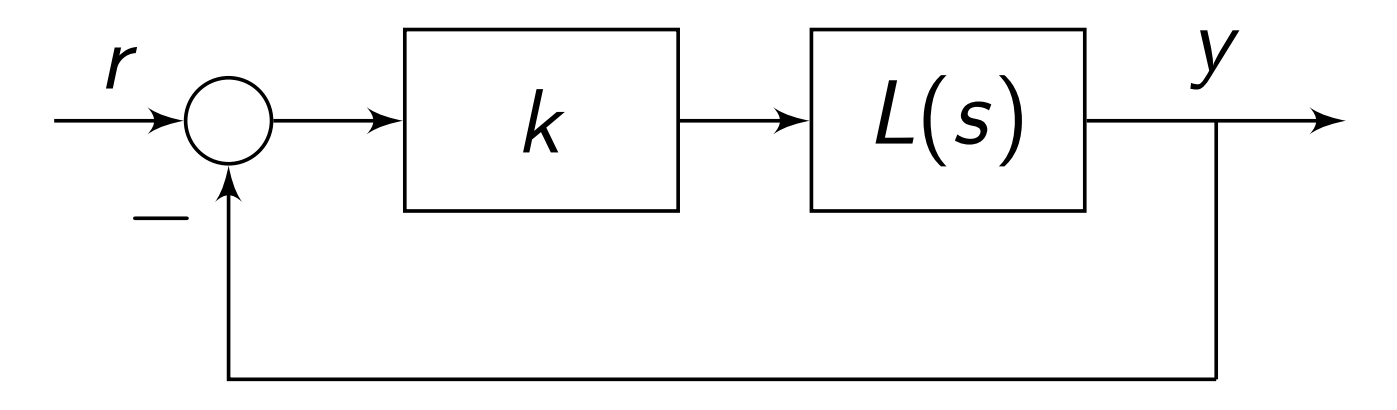
\includegraphics[width = \linewidth]{src/images/closed_loop.png}
\end{minipage}
\begin{align*}
    T(s) &= \frac{k L(s)}{1 + k L(s)} = \frac{k N(s)}{D(s) + k N(s)}
\end{align*}

\subsubsection{angle and magnitude rule}
\begin{align*}
    &\text{characteristic equation: } D(s) + kN(s) = 0\\
    &\Leftrightarrow \frac{N(s)}{D(s)} = L(s) = -\frac{1}{k}\\
    &\Rightarrow |L(s)| = \frac{1}{|k|} \quad \quad \quad
    \Rightarrow \angle(L(s)) = 
    \begin{cases}
        180 \text{° if } k > 0\\
        0 \text{° if } k < 0
    \end{cases}
\end{align*}

\subsubsection*{drawing the root locus}
\begin{itemize}
    \item closed-loop poles symmetric wrt real axis
    \item \# closed-loop poles = \# open-loop poles
    \item $k \rightarrow 0$: closed-loop poles approach open-loop poles
    \item $k \rightarrow \infty$: closed-loop poles approach open-loop zeros
    \item $n$ lines where $n =$ degree of D(s) or N(s), whichever greater
    \item no line crosses itself
    \item lines on the left of every odd numbered zero / pole (counting from right) (    o-----x    , x is 1st, o is 2nd, inverted for $k_{\text{bode}} < 0$)
    \item lines break out / in at 90°
    \item lines go to infinity along asymptotes with $\phi$ and centroid $c$ 
    \item $k < 0$: reverse rule 7 and add 180° to asymptotes
\end{itemize}
\begin{align*}
    n = \# \text{poles}, m = \# \text{zeros}, q = 0, 1, 2 \dots (n-m-1)\\
    \phi = \frac{2q + 1}{n-m} \cdot 180^{\circ}, c = \frac{\sum\text{finite poles} - \sum\text{finite zeros}}{n - m}
\end{align*}